\documentclass[12pt,a4paper]{article}

\usepackage{fancyhdr}
\usepackage{graphicx}
\usepackage{placeins}
\usepackage{adjustbox}


\begin{document}

\pagestyle{fancy}
\fancyhf{}
\chead{Short summary report}

\begin{table}[t]
\centering
\caption {rnaQUAST metrics for assembled transcripts. In each row the best values are indicated with \textbf{bold}. For the transcript metrics (rows 4, 5, 6, 9, 13, 26, 27, 28) we highlighted the best \textbf{relative} values i.e. divided by the total number of transcripts in the corresponding assembly.}
\begin{adjustbox}{width=1\textwidth}
\small
\begin{tabular}{|l*{11}{|r}|}
\hline
\textbf{METRICS/TRANSCRIPTS}                            & \textbf{Trinity}       & \textbf{Trans-ABySS}   & \textbf{Oases}         & \textbf{SOAPdenovo-Trans} & \textbf{IDBA-Tran}     & \textbf{Bridger}       & \textbf{BinPacker}     & \textbf{Shannon}       & \textbf{rnaSPAdes}     & \textbf{SPAdes}        \\ \hline\hline
\multicolumn{11}{l}{\bf DATABASE METRICS}                                                 \\ \hline
Genes                                                   & 57992                  & 57992                  & 57992                  & 57992                  & 57992                  & 57992                  & 57992                  & 57992                  & 57992                  & 57992                  \\
Avg. number of exons per isoform                        & 5.971                  & 5.971                  & 5.971                  & 5.971                  & 5.971                  & 5.971                  & 5.971                  & 5.971                  & 5.971                  & 5.971                  \\ \hline
\multicolumn{11}{l}{\bf BASIC TRANSCRIPTS METRICS}                                        \\ \hline
Transcripts                                             & 121575                 & 275008                 & 259024                 & 165909                 & 95730                  & 103284                 & 28888                  & 133199                 & 243604                 & 125233                 \\
Transcripts $>$ 500 bp                                  & 50409                  & 69717                  & 163070                 & 29135                  & 37135                  & 40276                  & \textbf{26809}         & 56849                  & 39548                  & 31264                  \\
Transcripts $>$ 1000 bp                                 & 31319                  & 37410                  & 115596                 & 15251                  & 16181                  & 23487                  & \textbf{22928}         & 35785                  & 21867                  & 15598                  \\ \hline
\multicolumn{11}{l}{\bf ALIGNMENT METRICS}                                                \\ \hline
Aligned                                                 & 121404                 & 274233                 & 257703                 & 165401                 & \textbf{95623}         & 103098                 & 28840                  & 133032                 & 241562                 & 124551                 \\
Uniquely aligned                                        & 116518                 & 263913                 & 229396                 & 162777                 & 94239                  & 96737                  & 25086                  & 125839                 & 236219                 & 110918                 \\
Multiply aligned                                        & 764                    & 2838                   & 1694                   & 1738                   & 595                    & 529                    & 58                     & 786                    & 1806                   & 7690                   \\
Unaligned                                               & 171                    & 775                    & 1321                   & 508                    & \textbf{107}           & 186                    & 48                     & 167                    & 2042                   & 682                    \\ \hline
\multicolumn{11}{l}{\bf ALIGNMENT METRICS FOR NON-MISASSEMBLED TRANSCRIPTS}               \\ \hline
Avg. aligned fraction                                   & 0.983                  & 0.982                  & 0.92                   & \textbf{0.995}         & 0.992                  & 0.975                  & 0.938                  & 0.981                  & 0.987                  & 0.986                  \\
Avg. alignment length                                   & 1040.875               & 534.402                & 1364.377               & 455.959                & 697.748                & 866.608                & \textbf{2505.426}      & 918.854                & 470.161                & 489.2                  \\
Avg. mismatches per transcript                          & 1.746                  & 0.753                  & 2.515                  & \textbf{0.443}         & 0.834                  & 1.487                  & 3.674                  & 1.426                  & 1.067                  & 0.72                   \\ \hline
\multicolumn{11}{l}{\bf ALIGNMENT METRICS FOR MISASSEMBLED (CHIMERIC) TRANSCRIPTS}          \\ \hline
Misassemblies                                           & 1294                   & 4769                   & 18893                  & \textbf{125}           & 203                    & 2509                   & 2649                   & 2605                   & 1219                   & 2042                   \\ \hline
\multicolumn{11}{l}{\bf ASSEMBLY COMPLETENESS (SENSITIVITY)}                              \\ \hline
Database coverage                                       & 0.178                  & \textbf{0.21}          & 0.201                  & 0.158                  & 0.15                   & 0.141                  & 0.102                  & 0.167                  & 0.173                  & 0.143                  \\
50\%-assembled genes                                    & 9849                   & \textbf{10377}         & 10258                  & 9406                   & 8675                   & 8480                   & 6728                   & 8889                   & 10186                  & 9154                   \\
95\%-assembled genes                                    & 3972                   & 3694                   & \textbf{4128}          & 3116                   & 776                    & 2722                   & 2585                   & 2562                   & 3628                   & 2790                   \\
50\%-covered genes                                      & 11338                  & 12053                  & 11355                  & 11234                  & 11103                  & 9903                   & 7054                   & 10747                  & \textbf{12078}         & 10454                  \\
95\%-covered genes                                      & 4999                   & 5157                   & \textbf{5252}          & 3965                   & 2003                   & 3286                   & 2879                   & 3761                   & 4691                   & 3454                   \\
50\%-assembled isoforms                                 & 14332                  & 17634                  & \textbf{17801}         & 11166                  & 10800                  & 10559                  & 8400                   & 12957                  & 12795                  & 10453                  \\
95\%-assembled isoforms                                 & 4696                   & 4004                   & \textbf{5115}          & 3225                   & 780                    & 2965                   & 2851                   & 2964                   & 3850                   & 2795                   \\
50\%-covered isoforms                                   & 16823                  & \textbf{22458}         & 20319                  & 14018                  & 14855                  & 12587                  & 8796                   & 16167                  & 15837                  & 12569                  \\
95\%-covered isoforms                                   & 5889                   & 5768                   & \textbf{6549}          & 4106                   & 2012                   & 3556                   & 3164                   & 4354                   & 4981                   & 3461                   \\
Mean isoform coverage                                   & 0.514                  & 0.464                  & 0.539                  & 0.385                  & 0.451                  & 0.435                  & \textbf{0.678}         & 0.529                  & 0.411                  & 0.422                  \\
Mean isoform assembly                                   & 0.461                  & 0.4                    & 0.491                  & 0.334                  & 0.38                   & 0.391                  & \textbf{0.654}         & 0.456                  & 0.36                   & 0.377                  \\ \hline
\multicolumn{11}{l}{\bf GeneMarkS-T METRICS}                                              \\ \hline
Predicted genes                                         & 33592                  & 50018                  & \textbf{96132}         & 17801                  & 25350                  & 23585                  & 18234                  & 41533                  & 23967                  & 18444                  \\ \hline
\multicolumn{11}{l}{\bf ASSEMBLY SPECIFICITY}                                             \\ \hline
50\%-matched                                            & 58201                  & 117092                 & 140767                 & 61852                  & 48574                  & 44187                  & \textbf{21827}         & 81027                  & 60734                  & 47018                  \\
95\%-matched                                            & 36579                  & 79703                  & 67696                  & 50736                  & 39613                  & 29804                  & 12271                  & \textbf{58664}         & 41312                  & 35929                  \\
Unannotated                                             & 47498                  & 128019                 & 60426                  & 85681                  & 35089                  & 40608                  & \textbf{1173}          & 38169                  & 159251                 & 61658                  \\
Mean fraction of transcript matched                     & 0.473                  & 0.42                   & 0.561                  & 0.372                  & 0.508                  & 0.44                   & \textbf{0.805}         & 0.609                  & 0.249                  & 0.319                  \\ \hline
\end{tabular}
\end{adjustbox}
\end{table}

\FloatBarrier
\clearpage
\lfoot{generated by rnaQUAST}

\begin{figure}[t]
\centering
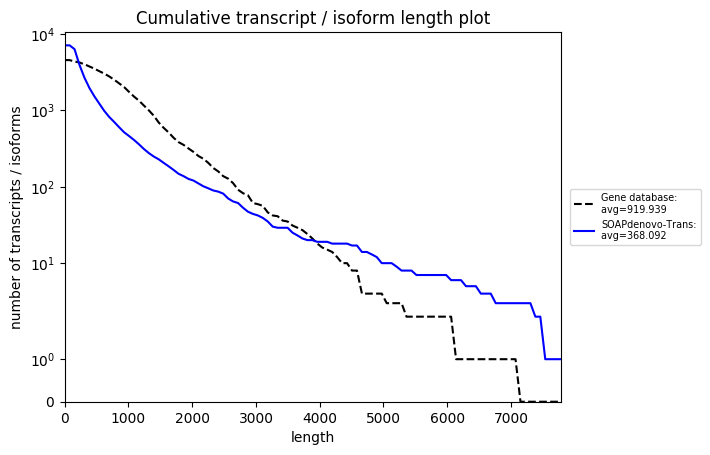
\includegraphics[width = \linewidth]{/mnt/dessertlocal/projects/transcriptome_assembly/review/evaluation/rna-quast/ebov_hsa_7h/comparison_output/transcript_length.png}
\caption{Plot showing cumulative transcript length distribution. Each point represents the number of transcripts in the assembly with the corresponding length or longer; black dashed line corresponds to the database isoforms; the plot is given in logarithmic scale.}
\end{figure}
\FloatBarrier
\clearpage


\begin{figure}[t]
\centering
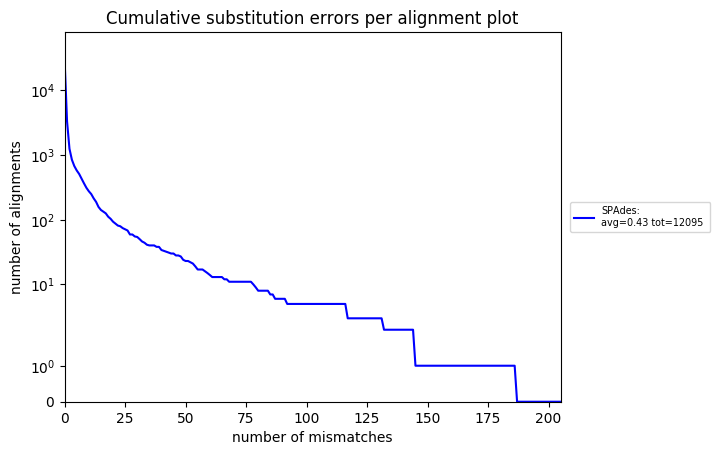
\includegraphics[width = \linewidth]{/mnt/dessertlocal/projects/transcriptome_assembly/review/evaluation/rna-quast/ebov_hsa_7h/comparison_output/mismatch_rate.png}
\caption{Plot showing cumulative substitution errors per alignment distribution. Each point represents the number of alignments with the corresponding number of mismatches or greater; the plot is given in logarithmic scale.}
\end{figure}
\FloatBarrier
\clearpage


\begin{figure}[t]
\centering
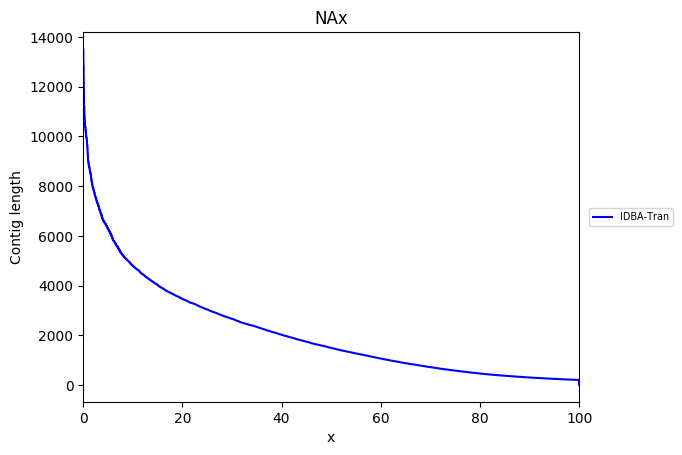
\includegraphics[width = \linewidth]{/mnt/dessertlocal/projects/transcriptome_assembly/review/evaluation/rna-quast/ebov_hsa_7h/comparison_output/NAx.png}
\caption{Nx plot for transcripts. Nx is a maximal number $N$, such that the total length of all transcripts longer than $N$ bp is at least $x\%$ of the total length of all transcripts.}
\end{figure}
\FloatBarrier
\clearpage


\begin{figure}[t]
\centering
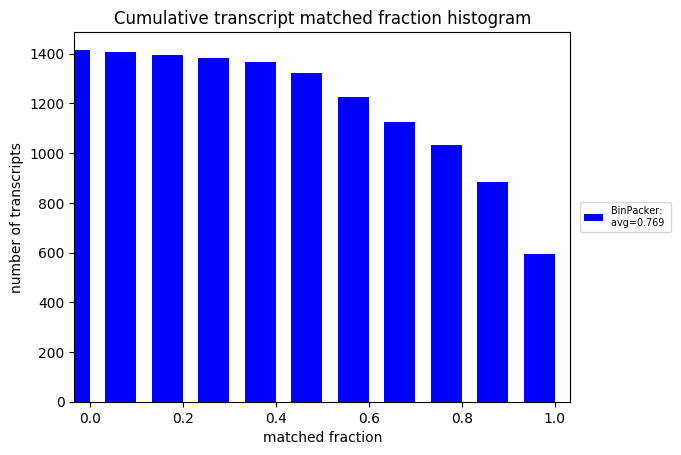
\includegraphics[width = \linewidth]{/mnt/dessertlocal/projects/transcriptome_assembly/review/evaluation/rna-quast/ebov_hsa_7h/comparison_output/x-matched.png}
\caption{Plot showing cumulative transcript match histogram. Each bar represents the number of transcripts with matched fraction equal to or greater than the value on $x$ axis; transcript matched fraction is calculated as the number of its bases covering an isoform divided by the transcript length.}
\end{figure}
\FloatBarrier
\clearpage


\begin{figure}[t]
\centering
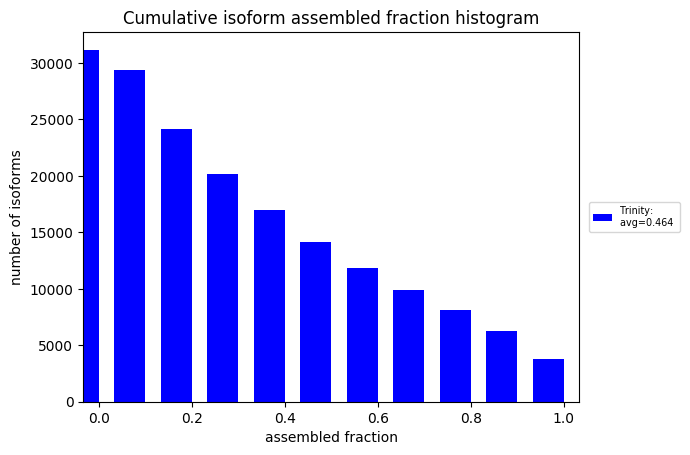
\includegraphics[width = \linewidth]{/mnt/dessertlocal/projects/transcriptome_assembly/review/evaluation/rna-quast/ebov_hsa_7h/comparison_output/x-assembled.png}
\caption{Plot showing cumulative isoform assembly histogram. Each bar represents the number of isoforms with assembled fraction equal to or greater than the value on $x$ axis; isoform assembled fraction is calculated as the maximum number of captured by single assembled transcript bases divided by the total isoform length.}
\end{figure}
\FloatBarrier
\clearpage


\begin{figure}[t]
\centering
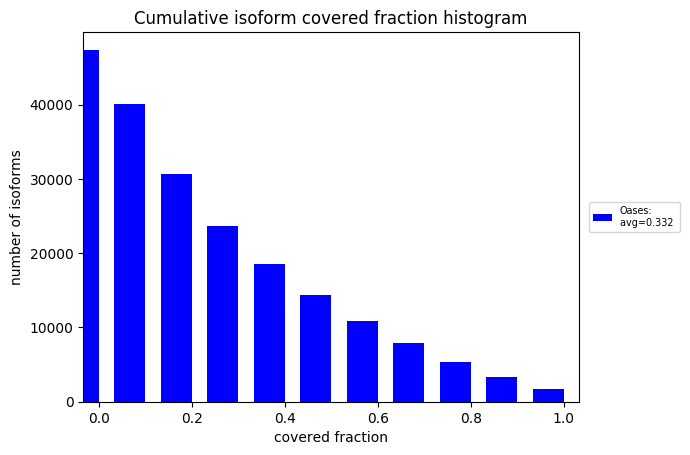
\includegraphics[width = \linewidth]{/mnt/dessertlocal/projects/transcriptome_assembly/review/evaluation/rna-quast/ebov_hsa_7h/comparison_output/x-covered.png}
\caption{Plot showing cumulative isoform coverage histogram. Each bar represents the number of isoforms with covered fraction equal to or greater than the value on $x$ axis; isoform covered fraction is calculated as the number of covered bases (by all transcripts in the assembly) divided by the total isoform length.}
\end{figure}
\FloatBarrier
\clearpage


\end{document}
